% -*- LaTeX -*-
% -*- coding: utf-8 -*-
%
% ~~~~~~~~~~~~~~~~~~~~~~~~~~~~~~~~~~~~~~~~~~~~~~~~~~~~~~~~~~~~~~~~~~~~~~~~~~~~~~
%
%                             michael a.g. aïvázis
%                      california institute of technology
%                      (c) 1998-2010  all rights reserved
%
% ~~~~~~~~~~~~~~~~~~~~~~~~~~~~~~~~~~~~~~~~~~~~~~~~~~~~~~~~~~~~~~~~~~~~~~~~~~~~~~
%

\lecture{Introduction to parallel programming models}{20100111}

% --------------------------------------
% generic parallel architecture
\begin{frame}[fragile]
%
  \frametitle{Impact of architecture on algorithm design}
%
  \begin{itemize}
%
    \item recall the five steps of parallel algorithm design
      \begin{itemize}
      \item identification of the parallelizable part, partitioning into fine grain tasks,
        examination of the task communication patterns, task coarsening, and mapping coarse
        tasks onto processors
      \end{itemize}
%
    \item and the layout of the generic parallel architecture:
%
  \end{itemize}
%
  \begin{figure}
    \centering
    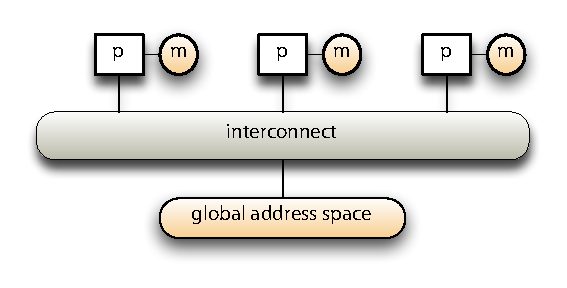
\includegraphics[width=.5\linewidth]{figures/generic-parallel-architecture.pdf}
    \label{fig:gpa-redux}
  \end{figure}
%
  \begin{itemize}
  \item let's move memory around and examine how this affects the programming model
  \item for a trivial but instructive problem
  \end{itemize}
%
\end{frame}

% --------------------------------------
% template
\begin{frame}[fragile]
%
  \frametitle{Parallel programming models}
%
  \begin{itemize}
%
  \item control
    \begin{itemize}
    \item how is parallelism {\em created}
    \item what is the {\em sequencing} of instruction streams in each task
    \item how do tasks {\em synchronize}
    \end{itemize}
%
    \item data address spaces
      \begin{itemize}
        \item what data is private to each task; what data must be shared
        \item how is logically shared data created, accessed or communicated, and synchronized
      \end{itemize}
%
    \item instruction sets
      \begin{itemize}
      \item what are the fundamental operations for process creation, communication,
        and synchronization
      \item which operations are {\em atomic}
      \end{itemize}
%
    \item cost
      \begin{itemize}
      \item how fast does it run
      \item are resources used efficiently
      \item how hard is it to code correctly
      \end{itemize}
%
  \end{itemize}
%
\end{frame}

% --------------------------------------
% template
\begin{frame}[fragile]
%
  \frametitle{Embarrassingly parallel: $p$ processor reduction}
%
  \begin{itemize}
%
  \item given a function $f$ and a sequence of numbers $S$ of length $N$, evaluate the sum
    \[
    s = \sum_{i=0}^{N-1}f(S_{i})
    \]
%
  \item parallel tasks: the function evaluations, the computation of partial sums
%
  \item strategy: assign $n/p$ numbers to each processor
    \begin{itemize}
      \item each processor performs $n/p$ evaluations of $f$
      \item each processor computes its own partial sum
      \item one (or all) of them collects the $p$ partial sums and computes $s$, the global sum
    \end{itemize}
%
  \item two classes of data
    \begin{itemize}
      \item logically shared:
        \begin{itemize}
        \item the global sum
        \item the input sequence $S$
        \end{itemize}
      \item logically private:
        \begin{itemize}
          \item the evaluations of $f$ on the local subsequence
          \item the local partial sums (?)
        \end{itemize}
    \end{itemize}
%
  \end{itemize}
%
\end{frame}

% end of file 
